\documentclass[main]{subfiles}

\begin{document}
\subsection{Modul To}
Efter at have målt switchen, som beskrevet i \cref{dataopsamling2}, konkluderes det, at system er hurtig nok til at måle et signal. Herefter måles laserstrålens waist, ved at logge den transmitterede intensitet som funktion af millimeterskrue. Dette ses på \cref{fig:graf3}.
\begin{figure}[H]
    \centering
    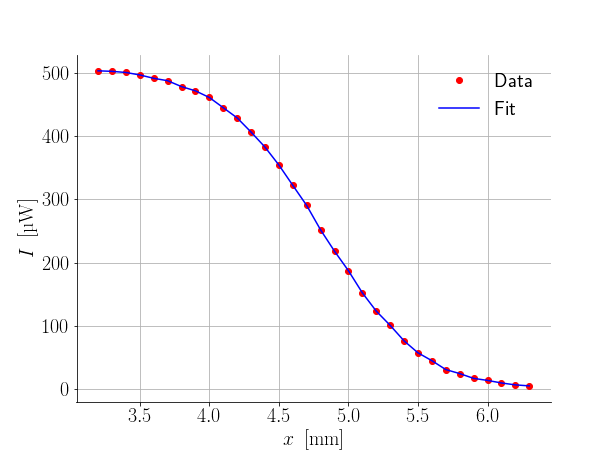
\includegraphics[width=\linewidth]{tegninger/graf3.png}
    \caption{}
    \label{fig:graf3}
\end{figure}
På \cref{fig:graf3} ses det at intensiteten af strålen falder mest når kniven er omkring midten af strålen, hvilket giver god mening idet at vi forventer at strålen fordeler sig omkring sin akse og vi dermed rammer mere af strålen omkring centrum. Umiddelbart ser figuren symmetrisk ud på den måde at den bevæger sig ensartet i bunden af grafen og toppen af grafen, hvilket understøtter forventningen om at strålen fordeler sig ensartet omkring laserens akse.
Ud fra figuren her kan waist, $w_0$ findes ved at indsætte nogle hjælpelinjer, netop da waist vil være forskellen i længde mellem de to punkter hvor intensiteten er 84\% og 16\% af max intensiteten.
\begin{figure}[H]
  \centering
  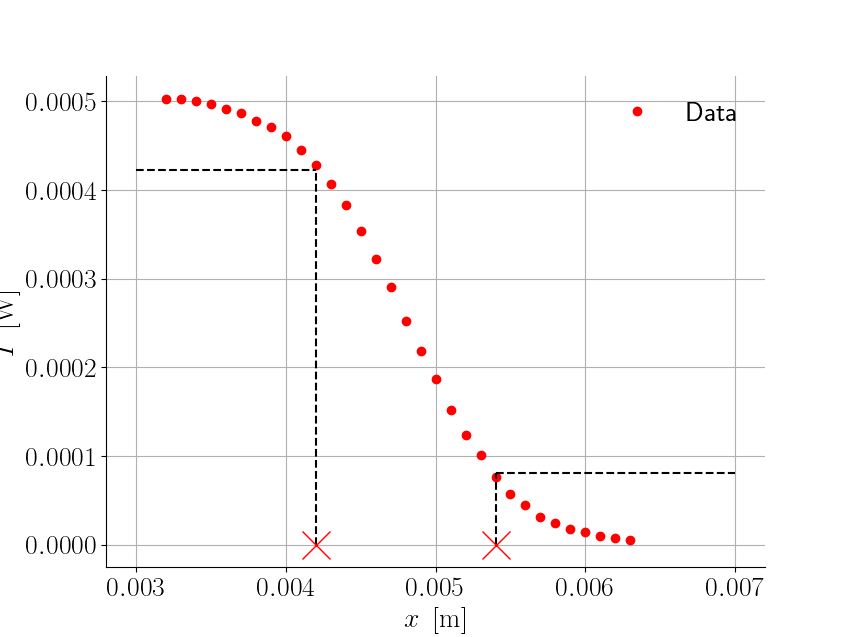
\includegraphics[width=\linewidth]{tegninger/graf_find_w.png}
  \caption{}
  \label{fig:graf_find_w}
\end{figure}
På \cref{fig:graf_find_w} ses de omtalte linjer og to røde krydser. De røde krydser indikerer punkterne hvor intensiteten er 84\% og 16\%. Det findes ud fra dette at afstanden mellem de to kryder bliver, $w_0 =\SI{1,2 \pm 0,1}{\milli\meter} $. Usikkerheden her er netop usikkerheden på længdemålingerne, som grundet millimeterskruen er $\SI{0,1}{\milli\meter}$. Det skal lige nævnes her at den omtalte waist her ikke er den sande waist idet at forsøgsopstillingen var lidt forkert, men at dette er metoden som bruges til at udregne waist.

Man kan også bestemme waist, $w_0$ ved at fitte til en funktion af typen som ses på \cref{eq:errorfunc}. Det har dog ikke været muligt grundet tekniske vanskeligheder.

Der er blevet bestemt tre andre waists som der er lavet risetime målinger med.
På \cref{fig:screenfigur} ses en måling af risetime med indstillede cursors. Denne måling er taget med en linse med brændvidde $F = \SI{100}{\milli\meter}$.
\begin{figure}[H]
  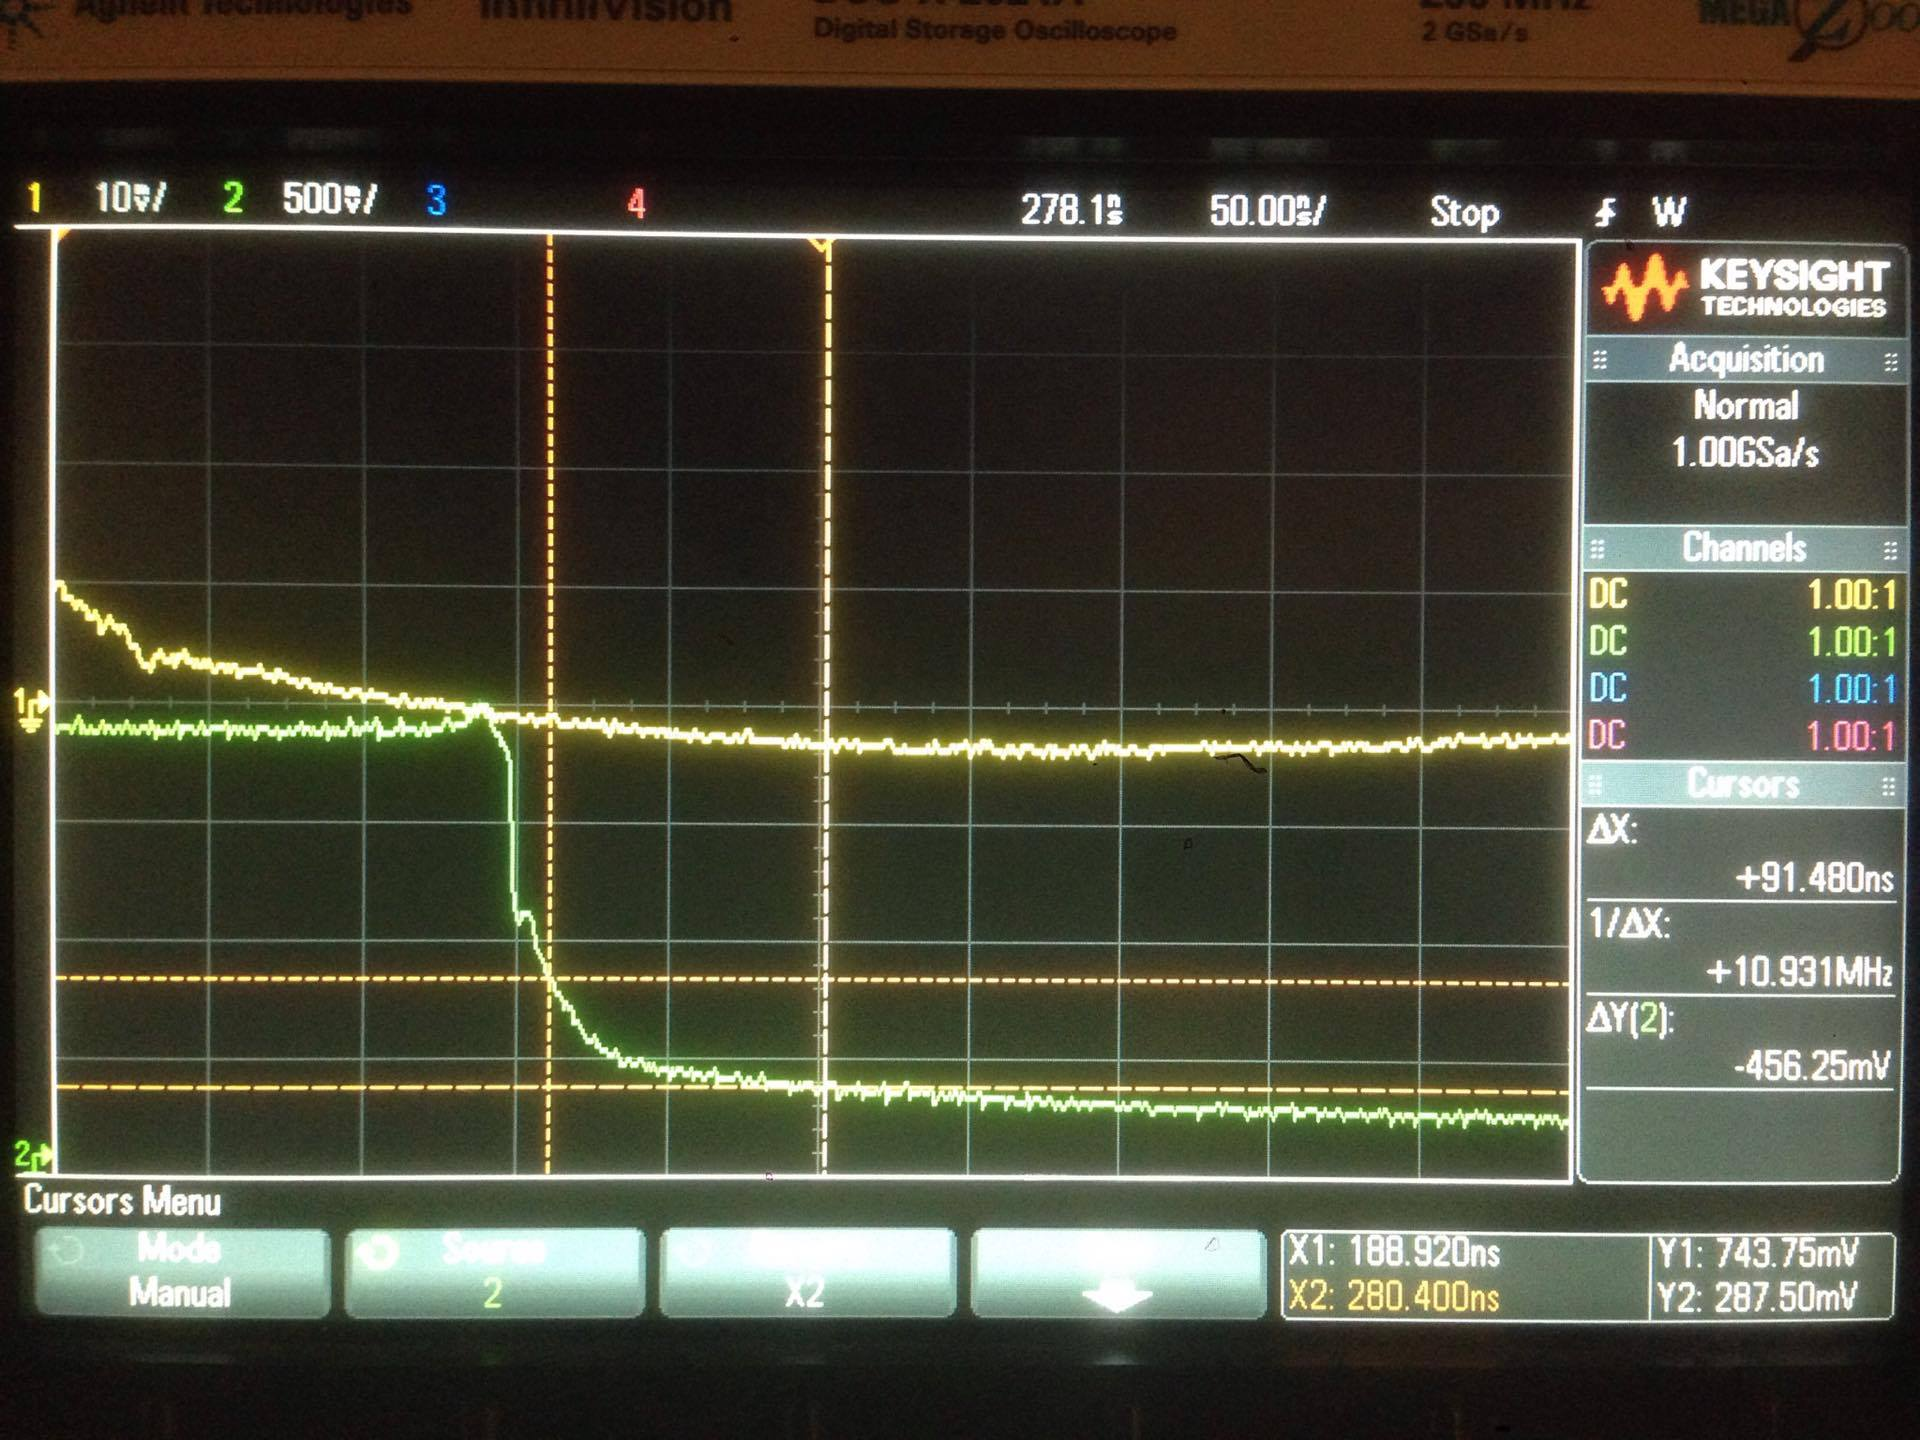
\includegraphics[width=\linewidth]{tegninger/screenfigur.png}
  \caption{}
  \label{fig:screenfigur}
\end{figure}
Denne måling er taget med en waist på $w_0 = \SI{0,213}{\milli\meter}$.

Der er yderligere taget målinger med fokallængder på $\SI{50}{\milli\meter}$ og $\SI{100}{\milli\meter}$.

Der er afbildet figurer med risetimes som funktion af waist ved disse fokallængder. Risetimes til hver waist er ikke den samme og dette er med til at give en ide om hvor usikker vores målinger her har været. Dette ses på \cref{fig:risetime_fig}
\begin{figure}[H]
  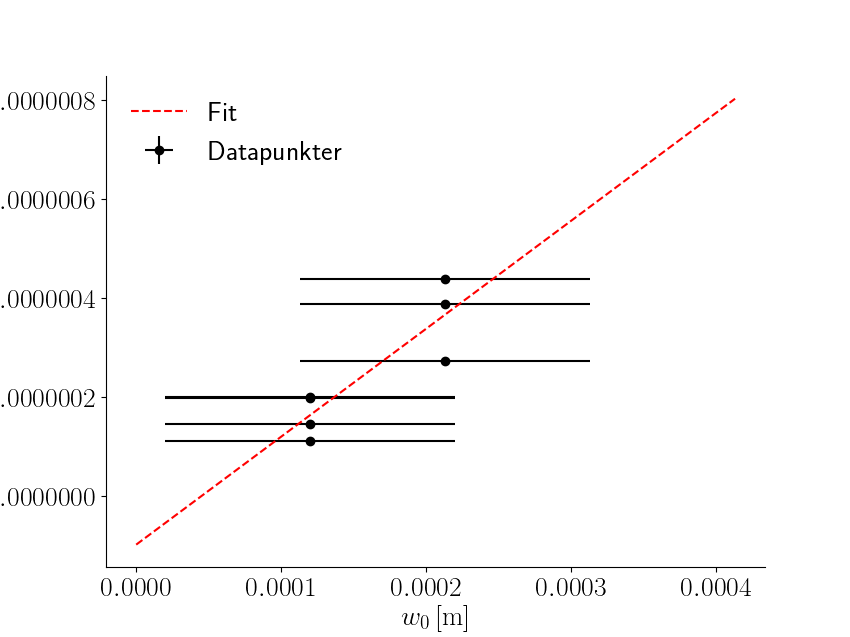
\includegraphics[width=\linewidth]{tegninger/risetime_fig.png}
  \caption{}
  \label{fig:risetime_fig}
\end{figure}
Det ses på \cref{fig:risetime_fig} at usikkerhederne på waist målingerne er ret store ift. til skalaen. Ud fra grafen her findes hældningen på kurven til at være, $\SI{0,002183}{\second\per\meter}$ og dette medfører da at den målte lydhastighed i krystallen her bliver: $v_{sound} = 586,3 \pm 138.5 \ \si{\meter\per\second}$. Usikkerheden på lydens hastighed er her fundet ud fra spredningen på fitteparametren, $k$ i et fit på typen $T_r = k\cdot w_0 +c $. Her er spredningen på denne parameter brugt til at finde usikkerheden på lydhastigheden ud fra ophobningsloven, altså ved:
\begin{equation}
  \nonumber sds(v_{sound}) = \sqrt{\left(\frac{0.64 \cdot 2}{k^2}\right)^2 \cdot sds(k)^2} = \SI{138.5}{\meter\per\second}
\end{equation}
Her skal det nævnes at der ikke burde være noget konstant led, men der er her brugt et for at sikre en god linje gennem datapunkterne. Den er ikke 0, men derimod $c = \SI{-9,82e-8}{\second}$ hvilket selvfølgelig er en meget lille værdi, men det er værdierne på vores data også.

\end{document}
